\chapter{Oversikt over valgte Teknologier}

\section{Publisering}
Ett av kravene til prosjektet var at nettsiden skal være så selvstendig som mulig. Det skal være minimalt med nedetid, serveren må kunne oppdateres uten manuelt inngrep og backup av database må foregå automatisk. Samtidig som å oppfylle dette burde selve hostingen være så billig som mulig. Derfor ble det noe moderne konseptet av Platform as a Service benyttet.

\subsection{Platform as a Service}
En Platform as a Service (PaaS) er et utviklings og distribusjons miljø basert i en skytjeneste \cite{ paas:azure}. En PaaS leverandør har som ansvar å levere og opprettholde en utviklings og distribusjons plattform for sine kunder. De har videre ansvaret på områdene rundt konfigurering, oppsett av servere og sikkerhet på server siden. Det er populært å referere til  PaaS leverandører som IT-avdelingen til produktet, som gjør at utvikleren kan fokusere mer på selve utviklingen enn oppsett av infrastrukturen som ligger under \cite[s. 10]{bachelor}

\subsection{Fordeler ved PaaS}
\subsubsection*{Spare Tid}
Utviklingen foregår direkte mot arkitekturen til den valgte skytjenesten, derfor vil man unngå forarbeidet rundt oppsett og installasjon av servere. Dersom en server hos PaaS leverandøren skulle gå offline, vil dette bli ordnet fortløpende av leverandøren, uten at man som kunde må gripe inn \cite[s. 9]{bachelor}.

\subsubsection*{Billig}
Samtidig som å levere mye i pakken, kan publisering vha. PaaS være billig. Dette kommer av at de aller fleste leverandørene bruker dynamisk ressursallokering. Det betyr at ressursene allokert til et prosjekt vil følge samme kurve som behovet. Ved lite eller ingen trafikk vil et prosjekt gå i dvalemodus og bli der helt til en forespørsel blir sendt til serveren. Man betaler kun for de ressurser som blir benyttet.

\subsection{Valg av PaaS Leverandør}
PaaS er fortsatt et moderne konsept, og man har mange muligheter ved valg av leverandør. Det er en enorm jobb å foreta en sammenlikning over de relevante mulighetene, derfor har jeg valgt å gå ut ifra et studie som jeg foretok under et bachelor prosjekt våren 2016 \cite[s. 18]{bachelor}. Her ble det utført en sammenlikning av 3 av de største PaaS leverandørene: Google Cloud Platform, Microsoft Azure og Amazon Web Services. 


\subsection*{Resultat}
Alle de tre nevnte leverandørene har et bredt utvalgt av muligheter på sine løsninger. Alle tilbyr et løfte av server tilgjengelighet på 99,95\% av tiden. De har gode tilkoblingsmuligheter i Europa og prisen er basert på tid og ressurser.

Men det er spesielt ett område de har unike løfter; Gratis Kvoter. \\
Microsoft Azure leverer kun gratis kvoter i form av trial account. Her får man ressurser for 200\$ som man kan benytte som man selv bestemmer, i løpet av de første 30 dager etter Trial Account blir opprettet.\\
Amazon  Web Services kommer utstyrt med 1 år ‘free tier’, som inneholder 5GB lagringsplass, 20 000 GET requests og 2 000 Put Requests.\\
Google Cloud Platform derimot tilbyr daglige gratis kvoter. Dette inkluderer bl.a. 28 Frontend Instance timer\footnote{Google Cloud Platforms ‘frontend instance’ blir opprettet ved at en applikasjon får en forespørsel, og denne instance vil være tilgjengelig for bruk de neste 15 minutter. Alle nye forespørsler i disse neste 15 minutter vil benytte samme frontend instance}, 1GB plass for lagring av logger, 1GB data inn og ut.


Ved å bruke Google Cloud Platforms gratis kvoter, vil man kunne ha hosting av mindre trafikkerte nettsider bortimot gratis, og man behøver kun betale for databasen.\\
\textbf{Valg: Google Cloud Platform}



\newpage
\section{Programmeringsspråk og Rammeverk}
Med dette prosjektet ville jeg videreutvikle min kompetanse innen bruken av web-applikasjons rammeverket Django, basert på programmeringsspråket Python. 
\subsection{Python}
Python er et skriptingspråk utviklet av nederlandske Guide van Rossum. Den tidligste versjonen kom frem i 1996 og det har stadig vært i utvikling siden. Python har et formål om å gjøre kode leselig og gjenbrukbar, og har et mindre fokus på ren hastighet. Utover dette har Python et fokus på å gjøre utviklingen, og debuggings fasene av prosjekter så raskt som mulig \cite[s. 11]{bachelor}.
\subsection{Django}

\begin{wrapfigure}{r}{4.5cm}
\caption[Django Oversikt]{Stegene Django kjører gjennom ved et HTML request. }\label{wrap-fig:1}
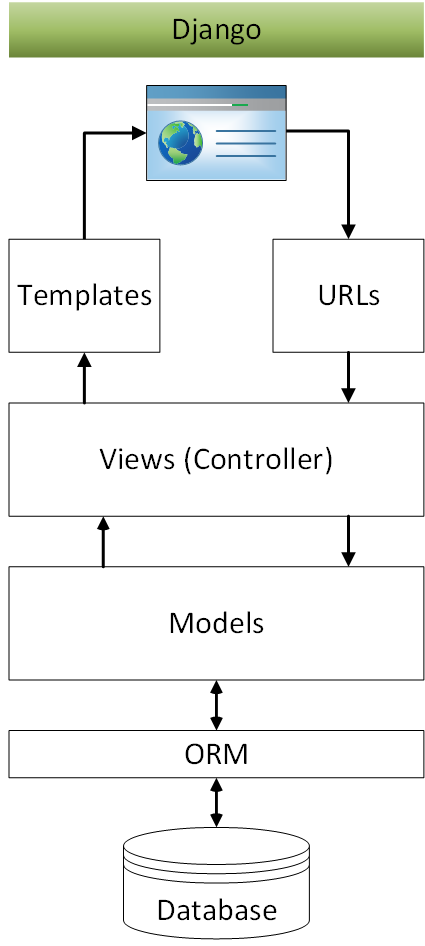
\includegraphics[width=4.5cm]{Bilder/django.png}
\end{wrapfigure}

Django er et web-applikasjons rammeverk som kommer levert med en ‘batterier inkuldert' filosofi. Dette betyr at vanlig funksjonalitet som ofte blir benyttet i en web sammenheng blir levert med i grunnpakken til Django. Dette inkluderer bruker-system, URL routing, template system, administrasjons system og database object-relational mapper (ORM) \cite{django:what}.





På figur \ref{wrap-fig:1} kan man se en oversikt over hvordan Django håndterer et HTML request. 

Først vil den tyde hvilke URL som kommer inn. Django inneholder et register over tilgjengelige URL som kan benyttes vha. regular expressions. Den vil sjekke dette registeret og finne hvilken funksjon (view) som tilhører den innkommende URL.

Den korresponderende funksjon i view vil nå håndtere data fra HTML requestet, dette innebærer å sjekke om det er et POST eller GET request, og hente ut eventuell data med henyn til dette. 

Data vil bli hentet vha. Djangos Modeller, som er et objekt orientert metode å fremstille den tilkoblede databasen. Når det er klart hvilke data som skal hentes, vil Djangos ORM konvertere Djangos Database API til SQL Query. Den data som resulterer fra spørringen vil bli returnert tilbake til view.

Til slutt vil view samle data og generere den tilhørende template (html), som videre sendes tilbake til browseren.



\section{Front-end}
\subsection{Bootstrap}
Bootstrap ble først laget av en designer og utvikler hos Twitter i 2010, og har fått stort følge siden. Det er i dag ett av de største og mest populære front-end rammeverkene i verden. Da det er så mye brukt, vil det da være et større følge aktive brukere på nettsider som stackoverflow.com, som videre gjør det mer attraktivt å bruke.

\subsubsection*{Skalerbart}
Boostrap kommer utstyrt med et Grid system. Dette systemet er basert på å dele opp skjermen inn seksjoner, basert på skjermstørrelsen. Dette gir muligheten av å kunne spesifisere hvordan et element skal oppføre seg i forhold til skjermstørrelsen, dette resulterer i en nettside som fungerer like godt på smartphones, tablets og PCer.

\subsubsection*{Komponenter}
Rammeverket kommer med en hel rekke komponenter som kan benyttes.  Dette gjelder bl.a. en rekke valg innen navigasjonsmenyer, input bokser, knapper etc. Disse komponentene er videre fult mulig å redigere vha. CSS.

\newpage
\section{Verktøy}
\begin{description}
\item[GitHub]ble benyttet som versjons kontroll underveis i utviklingen. For hver nye feature som skulle introduseres, ble dette utviklet på en egen branch. Når utviklingen av en ny feature fungerte som planlagt, skulle den testes grundig før den ble pushet over på Master branch.
\item[Google App Engine SDK.] Google Cloud Platform kommer utstyrt med en SDK når man skal arbeide mot Google App Engine. Denne SDK inneholder et lokalt utviklingsmiljø som kjører på samme infrastruktur som det benyttet ved hostingen. Man får også publisering og administrasjons muligheter direkte vha. enkel GUI. Denne har hovedsakelig blitt brukt som et test område underveis i utviklingen, samt. Publisering av nyere versjoner etter hvert som nettsiden har blitt oppdatert.
\item[JetBrains PyCharm] har blitt brukt som IDE. Denne inneholder en bred rekke hjelpemidler for å gjøre utviklingsprosessen smidigere. Den støtter både utvikling av Django prosjekter og html/css/javascript. I tillegg har den et godt system for autocomplete av kode, og vil generere hint for forbedringer av bl.a. navn på funksjoner, indentering og sørger for at all kode benytter samme navn konvensjon.
\item[LateX.]Under rapportskrivingen har typesettingssystemet LateX blitt brukt får å generere dokumentet. Dette systemet hjelper med å skape en god utforming av hele dokumentet, som gir bedre muligheter for å fokusere på selve skrivingen. LateX gir et såkalt WYSIWYM (What You See Is What You Mean), som beskriver en form for skriving hvor det resulterende dokument bedre representerer den faktiske informasjonen man arbeider med.



\end{description}

